\chapter{Implementacja}
\label{cha:implementacja}
W ramach niniejszej pracy magisterskiej stworzono grę elektroniczną, w~której miał zostać wykorzystany przygotowywany prototyp interfejsu do  odczytu zmianów stanów emocjonalnych i~zachowań gracza. Na podstawie analizy silników do tworzenia gier przeprowadzonej w~rozdziale~\ref{cha:specyfikacja} zdecydowano się na wykorzystanie silnika Unity. Głównym powodem takiej decyzji była przede wszystkim ilość materiałów o~tematyce tworzenia gier przy pomocy właśnie silnika Unity, a~także dostępność rozwiązań, które pozwalały na prostą komunikację z~urządzeniami opisanymi w~rozdziale~\ref{cha:architektura}. 

\section{Podstawowe założenia}
Zanim rozpoczęto implementację gry, zostały określone założenia i~wymagania implementacyjne i~projektowe, według których następnie została zbudowana gra:
\begin{enumerate}
	\item Gra powinna zawierać mechaniki afektywne, które modyfikują rozgrywkę w~zależności od zachowania lub stanu emocjonalnego gracza.
	\item Jednym z~elementów implementacyjnych powinien być moduł umożliwiający komunikację z~urządzeniami opisanymi w~rozdziale~\ref{cha:architektura}. Moduł powinien także komunikować się z~serwerem zawierającym moduł do predykcji emocji oraz w~sposób prosty udostępniać zmiany stanu emocjonalnego użytkownika i~jego zachowań. 
	\item Gra powinna mieć możliwość wyboru jednego z~dwóch trybów gry: podstawowego, zawierający standardowe mechaniki gry, oraz wersję afektywną.
	\item Rozgrywka powinna być powtarzalna, tak aby w~trakcie przeprowadzania badań, każdy z~uczestników mógł doświadczyć tych samych elementów gry.
\end{enumerate}

\section{Implementacja gry}
%Opis gry, które elementy za co odpowiadają
Ponieważ przygotowywana gra miała być wykorzystana do przeprowadzenia eksperymentów w~celu ewaluacji opracowanego rozwiązania, zdecydowano, że będzie to gra jednoosobowa. W~trakcie rozgrywki gracz wciela się w~rolę kapitana statku kosmicznego, który musi walczyć z~przeciwnikami, aby przeżyć. Jego zadaniem jest sterowanie statkiem i~pokonanie jak największej liczby przeciwników przy pomocy dostępnego wyposażenia. Rozgrywka podzielona jest na poziomy, w~których trakcie gracz musi zdobyć określoną liczbę punktów. Na każdym z~poziomów dookoła statku generowanych jest kilka rodzajów wrogich statków, których schemat i~szybkość generowania są zróżnicowane w~zależności od poziomu. Z~każdym kolejnym poziomem pojawiają się nowe rodzaje jednostek, które mogą nie tylko wlatywać w~gracza lub do niego strzelać pojedynczymi pociskami, ale również wybuchać w~jego pobliżu, posiadać większą wytrzymałość lub strzelać innymi rodzajami pocisków. Każdy z~przeciwników ma także przypisaną ilość punktów, która jest dodawana do puli po zniszczeniu go. Aby przejść do kolejnego poziomu, gracz musi zebrać odpowiednią liczbę punktów.

Gracz posiada ograniczoną liczbę punktów życia, która zwiększa się po przejściu każdego z~poziomów. Aby urozmaicić rozgrywkę, dookoła gracza mogą pojawić się także wzmocnienia w~postaci innych broni oraz elementów leczących. Innym elementem mającym mocno wpłynąć na rozgrywkę jest moc specjalna, która umożliwia graczowi wypuszczenie fali w~kształcie okręgu, która natychmiastowo niszczy wrogie statki. Ponieważ umiejętność ta bardzo ułatwia rozgrywkę, gracz jest w~stanie użyć jej jedynie co określony czas. 

Aby wyrównać poziom gry i~nie znudzić gracz powtarzalną rozgrywką, każdy z~poziomów posiada także dodatkowy tryb, który jest trudniejszy niż podstawowa rozgrywka. Tryb ten jest uruchamiany na pewien określony czas po spełnieniu specjalnych warunków, które w~zależności od wersji gry są inne. W~trakcie trwania trybu trudnego schemat generowania przeciwników jest zmieniany na ich trudniejsze wersje, posiadające większą ilość życia i~inne umiejętności. Zmienia się także szybkość generowania przeciwników, która zostaje podwojona.

Cała gra została stworzona w~stylu dwuwymiarowym. Na rysunku~\ref{fig:ui} przedstawiony został fragment przykładowej rozgrywki. Oznaczone elementy interfejsu użytkownika to kolejno:
\begin{enumerate}
	\item \textbf{Pasek wskazujący poziom życia bohatera}. Warto zwrócić uwagę na brak oznaczenia dokładnej ilości punktów życia. Ukrycie tej informacji zmusza użytkownika do kontrolowania poziomu życia w~trakcie gry, a~także do unikania wszystkich przeciwników, niezależnie od tego, jakie obrażenia zadają.
	\item \textbf{Ikony aktualnie wybranej broni i~dostępności mocy specjalnej}. Służą one przede wszystkim jako elementy informacyjne. Wskazanie aktualnie wybranej broni pozwala graczowi między innymi na zorientowanie się, czy wzmocnienie w~postaci innego typu pocisków jest lepsze od aktualnie posiadanego. Ikona mocy specjalnej natomiast jest nie tylko wskazaniem jej dostępności. W~trakcie czasu odnowienia mocy specjalnej ikona ta spełnia funkcję orientacyjnego licznika, który wskazuje użytkownikowi, kiedy ponownie będzie mógł z~niej skorzystać.
	\item \textbf{Ilość punktów zdobytych przez gracza oraz pasek postępu dla danego poziomu}. Podobnie jak w~przypadku ilości punktów życia, pasek postępu wskazuje jedynie orientacyjny postęp gracza na danym poziomie, dzięki czemu użytkownik nie jest do końca pewien, kiedy ukończy poziom. Z~drugiej strony wyświetlana jest suma punktów zdobytych w~trakcie całej rozgrywki, co stanowi pewnego rodzaju motywację dla gracza, aby zdobyć jak najwyższy wynik.
\end{enumerate}

\begin{figure}
	\centering
	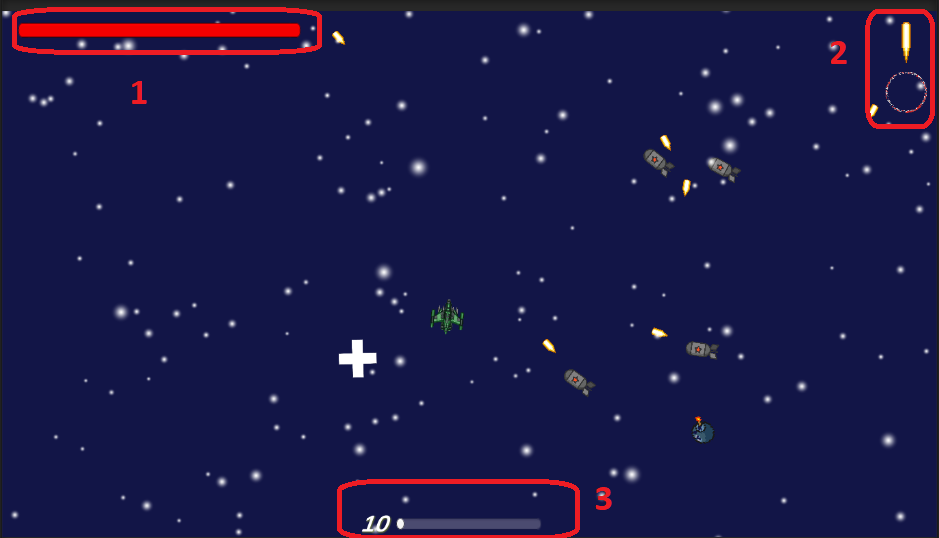
\includegraphics[width=0.7\linewidth]{images/ui.png}
	\caption{Ekran gry z~oznaczonymi elementami interfejsu użytkownika}
	\label{fig:ui}
\end{figure}

Tak jak zostało wspomniane na początku rozdziału, do implementacji gry wykorzystano silnik Unity. W~momencie tworzenia projektu gry zdecydowano się na użycie wersji 2018.3.0f2, która jest przeznaczona do tworzenia gier na systemy operacyjne oparte o~architekturę 64-bitową. Ponieważ projektowanie gier przy pomocy tego silnika jest oparte na tworzeniu obiektów, które są wprowadzane w~interakcje pomiędzy sobą, a~logika za to odpowiadająca zawarta jest w~skryptach dołączanych do obiektów, zdecydowano się na stworzenie hierarchii, w~której pierwszym poziomem są poszczególne elementy rozgrywki w~postaci obiektów tworzonych na scenie gry, drugim natomiast są skrypty odpowiadające za logikę danego obiektu lub innych elementów gry takich jak interfejs użytkownika czy postępy gracza. Do obiektów stanowiących główne elementy świata gry należą:
\begin{enumerate}
	\item \textbf{Player} reprezentujący statek, którym kieruje gracz. Poza elementami graficznymi zawiera on następujące skrypty związane ze sterowanym statkiem:
	\begin{itemize}
		\item \textbf{PlayerController}, opisujący sposób poruszania się kontrolowanego statku. Przy jego pomocy ustawiana są także szybkość poruszania się oraz czas potrzebny na wyhamowanie statku.
		\item \textbf{PlayerShooter}, odpowiadający za logikę strzelania przy pomocy wybranej broni, a~także za użycie mocy specjalnej. Jej głównym zadaniem jest zarządzanie tworzeniem pocisków i~aktywacji animacji oraz dźwięków związanych ze strzałem lub aktywacją mocy specjalnej. Skrypt odpowiada także za integrację z~elementami interfejsu użytkownika odpowiedzialnymi za wyświetlanie aktualnie używanej broni i~dostępności mocy specjalnej. Skrypt umożliwia także zmianę aktualnie używanej broni oraz zarządzanie parametrem czasu odnowienia mocy specjalnej. 
		\item \textbf{Player}, odpowiadający za kontrolowanie życia postaci. Mowa tutaj nie tylko o~zmniejszaniu życia po przyjęciu obrażeń lub zwiększaniu podczas leczenia bohatera, ale również ustawianiu nowej wartości maksymalnej ilości punktów życia po zakończeniu poziomu. Skrypt ten zarządza elementem interfejsu użytkownika odpowiedzialnym za wyświetlanie aktualnej ilości punktów życia. Kontroluje także wywołanie animacji i~dźwięków uruchamianych po śmierci bohatera, a~także oddelegowanie akcji odpowiedzialnych za zatrzymanie gry do obiektów sterujących rozgrywką.
	\end{itemize}

	\item \textbf{Obiekty reprezentujące przeciwników}. Każdy z~nich różnił się przypisanymi elementami graficznymi oraz skryptami, które mogą różnić się w~zależności od typu przeciwnika. Do skryptów sterujących logiką przeciwników należą:
	\begin{itemize}
		\item \textbf{Enemy}, odpowiadający przede wszystkim za zarządzanie poziomem życia przeciwnika, zmniejszaniu go po zadaniu obrażeń przez gracza, zmianie elementów graficznych w~zależności od ilości punktów życia przeciwnika, oraz za wywołanie animacji i~dźwięków mających nastąpić po śmierci przeciwnika. Skrypt posiada także parametr związany z~ilością obrażeń zadawanych podczas zderzenia z~graczem i~zarządza samą akcją kolizji, zabierając graczowi ustaloną ilość punktów życia.
		\item \textbf{EnemyMovement}, odpowiadający za sposób poruszania się przeciwnika. W~zależności od typu wroga, skrypt zarządza czy ma się on zbliżać do gracza, okrążać go, czy może stać w~miejscu. Zawiera on parametry dotyczące szybkości przeciwnika, maksymalnej odległości od gracza, oraz dystansu od niego, na jakim część przeciwników ma się zatrzymać.
		\item \textbf{EnemyShooter}, odpowiadający za kontrolę strzałów przeciwnika, ich szybkość, stworzenie pocisków oraz wywołanie efektów dźwiękowych strzału. Skrypt ten jest przypisywany wyłącznie do przeciwników typu strzelającego.
		\item \textbf{EnemyBomber}, zarządzający logiką wybuchu przeciwnika. Kontroluje przede wszystkim zadanie graczowi obrażeń i~odepchnięcie innych przeciwników, jeśli znajdują się w~zadanej przez parametr odległości. Odpowiada także za uruchomienie animacji oraz dźwięku związanych z~odliczaniem do wybuchu.
	\end{itemize}
	
	\item \textbf{Obiekty reprezentujące wzmocnienia, które gracz może zdobyć w~trakcie rozgrywki}. Poza elementami graficznymi, w~zależności od rodzaju wzmocnienia, każdy z~nich ma przypisany do siebie następujące skrypty:
	\begin{itemize}
		\item \textbf{PowerUp}, odpowiadający za wywołanie efektu wzmacniającego gracza, oraz ciągły obrót obiektu wzmocnienia. Jest to skrypt abstrakcyjny, co oznacza, że nie jest przypisany bezpośrednio do obiektu, a~stanowi bazę dla skryptów, które mogą rozszerzać jego zachowanie. W~tym przypadku rozszerzeniem jest funkcja, która odpowiada za nałożenie efektu wzmacniającego na gracza.
		\item \textbf{HealthPowerUp}, będący rozszerzeniem skryptu PowerUp. W~ramach wzmocnienia skrypt przywracał pewną ilość punktów życia określoną przez parametr.
		\item \textbf{WeaponPowerUp}, będący rozszerzeniem skryptu PowerUp. Wzmocnienie w~tym przypadku polegało na zmianie broni gracza na tę, która była przypisana do wzmocnienia w~formie parametru.
	\end{itemize}
\end{enumerate}

Poza wyżej wymienionymi elementami, które stanowią część gry widoczną dla gracza, stworzone zostały elementy będące częścią menu głównego, a~także obiekty zarządzające nieposiadające reprezentacji graficznej. Do każdego z~nich został przypisany skrypt, który odpowiadał za kontrolowanie innych elementów rozgrywki:
\begin{itemize}
	\item \textbf{MainMenu}, zawierający funkcje, które uruchamiały oraz zamykały grę. W~ramach funkcji inicjującej rozgrywkę skrypt uruchamiał animacje wyświetlające ekran powitalny, a~następnie rozpoczynający faktyczną rozgrywkę.
	\item \textbf{PowerUpGenerator}, odpowiadający za generowanie obiektów wzmocnień w~trakcie gry. Kontrolował on tworzenie wybranego wzmocnienia w~losowo wybranej pozycji w~określonej odległości od gracza. Ilość wzmocnień znajdujących się  w~trakcie gry jest ograniczona, aby użytkownik odczuł, że są to elementy wyjątkowe. Wartość ta, wraz z~częstotliwością generowania wzmocnień i~odległością od gracza, w~jakiej obiekty mają być generowane, sterowane są przez parametry skryptu. 
	\item \textbf{EnemySpawner}, wykorzystywany do zarządzania logiką odpowiadającą za generowanie przeciwników w~świecie gry. Skrypt ten posiadając określoną w~parametrze listę szablonów przeciwników, którzy mają być generowani, co pewien czas tworzy każdego z~przeciwników w~formie fali. Każdy z~nich pojawia się w~losowo dobranych miejscach. Częstotliwość fal i~odległość, w~jakiej przeciwnicy są generowani od gracza, określane są poprzez parametry skryptu.
	\item \textbf{GameManager}, zarządzający zatrzymywaniem rozgrywki, oraz sterowaniem elementami po zakończeniu gry. Skrypt ten kontrolował flagi blokujące wszystkie inne obiekty w~przypadku zakończenia gry. Odpowiadał on także za wywołanie animacji wyświetlanych po śmierci gracza, zmianę sceny w~przypadku wyjścia z~gry, czy jej ponowne uruchomienie w~przypadku chęci ponownego rozpoczęcia rozgrywki.
	\item \textbf{Progress}, będący miejscem sterującym postępami gracza. Przy jego pomocy gromadzone są punkty zdobyte w~trakcie rozgrywki. Po zdobyciu punktów skrypt sprawdza, czy przekroczony został wynik wymagany do ukończenia poziomu. Jeżeli tak to usuwa wszystkie obiekty przeciwników i~pociski ze sceny, a~następnie w~zależności od tego, czy dany poziom był ostatni, uruchamia funkcje odpowiadające za zakończenie gry, lub przejście do kolejnego poziomu. W~przypadku końca rozgrywki, skrypt uruchamia animację wyświetlającą gratulacje dla gracza, a~następnie oznacza rozgrywkę jako zakończoną przy pomocy flagi ze skryptu GameManager. W~przypadku przejścia na kolejny poziom aplikowana jest nagroda w~postaci zwiększonych punktów życia, a~następnie ładowany jest kolejny poziom. Jednocześnie, niezależnie od tego, czy gracz ukończył poziom, aktualizowane są elementy interfejsu wyświetlającego ilość punktów gracz oraz sprawdzany jest warunek wymagany do uruchomienia trybu trudnego gry. Jeżeli tak, to lista generowanych przeciwników zostaje zmieniona na trudniejszą wersję, a~częstotliwość fal zostaje podwojona. W~ramach parametrów skryptu należy wyróżnić warunki uruchomienia trybu trudnego i~czas jego trwania, a~także listę poziomów w~grze. Ten ostatni parametr stanowi tak naprawdę główny rdzeń rozgrywki, ponieważ zawiera w~sobie szablon każdego z~poziomów, na który składają się: listy przeciwników, którzy mają być generowani, zarówno w~wersji klasycznej, jak i~trudnej, częstotliwość fal wrogów, wynik wymagany do ukończenia poziomu, liczba punktów życia dodana graczowi po jego ukończeniu, a~także flaga oznaczająca czy dany poziom jest ostatnim.
\end{itemize}

Wszystkie powyższe elementy stanowiły bazę dla podstawowej wersji gry. Parametry każdego z~obiektów zostały dobrane tak, aby gracz odczuwał postęp, który ma doprowadzić go ostatecznie do końca gry. Struktura projektu została zachowana w~formie dwóch scen, jednej odpowiedzialnej za menu gry, druga będąca sceną, w~której odbywała się faktyczna rozgrywka. Tak jak to zaznaczono podczas opisywania skryptów, całość gry rozgrywa się w~jednej scenie. Wynika to przede wszystkim z~powtarzalności poziomów, które różnią się wyłącznie parametrami. 

Ostatnim etapem tworzenia podstawowej wersji gry było dostosowanie sterowania do wykorzystywanego kontrolera Dualshock 4. Ponieważ Unity dla każdej z~gier może mieć zdefiniowaną listę nazw odpowiadającym danym przyciskom lub elementom, które mają pewien zakres działania, poza przystosowaniem standardowych nazw do odpowiednich przycisków na kontrolerze, dodane zostały osie, które zawierały w~sobie odczyty z~prawego analoga kontrolera. Pozwoliło to na wykorzystanie go do kontrolowania kierunku, w~który chciał spojrzeć gracz.

\section{Odczyt danych fizjologicznych i~zmian emocji}
Opis elementów do odczytu emocji i~EMG, odczyty z~cheststrapa, komunikacja z~serwerem

\section{Domknięcie pętli afektywnej}
Mechaniki, reakcja na konkretne emocje i~odczyty z~EMG, jak działa wersja bez emocji